\begin{problem}{Searching a Graph}

\begin{table}[h]
\centering
\begin{minipage}{0.45\linewidth}
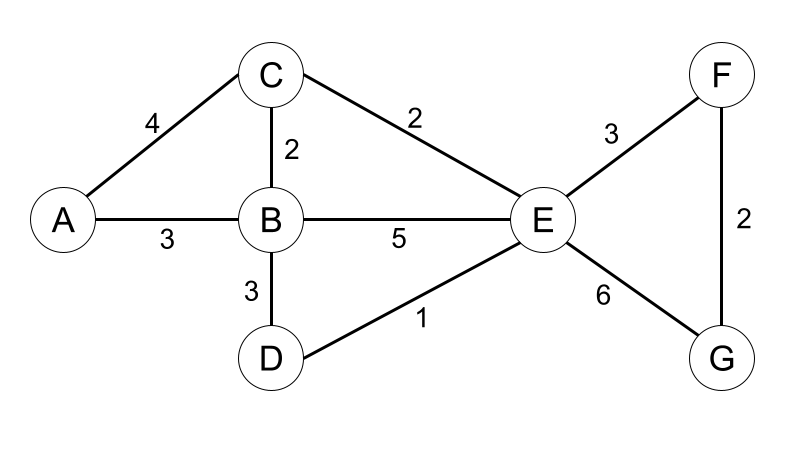
\includegraphics[scale=0.3]{figures/graph2.png} 
\end{minipage}
\hspace{1.5cm}
\begin{minipage}{0.45\linewidth}
\begin{tabular}{|l|l|l|}
\hline
Node & $h_1$ & $h_2$\\
\hline
A &12 &11\\
B &6 &7\\
C &9 &6\\
D &3 &4\\
E &3 &5\\
F &2 &1\\
G &0 &0\\
\hline
\end{tabular}
\end{minipage}
\end{table}

Consider the graph shown above. A is the start state and G is the goal state. The costs for each edge are shown on the graph. The graph is bi-directional so each edge can be traversed from either direction. Please refer to the search algorithms \textbf{exactly as presented on the lecture slides} as the ordering of the actions matters.

\begin{question}[15]
For each of the following \textbf{graph search} strategies, mark with an X which (if any) of the listed paths it could return. Note that for some search strategies the specific path returned might depend on tie-breaking behavior. In any such cases, make sure to mark \textbf{all} paths that could be returned under some tie-breaking scheme. If a graph search strategy returns a path not listed, \textbf{write out the correct path} in the \textit{Other} column.\\


\begin{table}[h]
\begin{center}
\begin{tabular}{|l|l|l|l|l|}
\hline
Algorithm & A-C-E-G & A-C-E-F-G & A-B-D-E-F-G & Other\\
\hline
UCS & \begin{minipage}{2cm}~\\(i)\quad\solution{}{\Threeai}~\\~\\\end{minipage} &
\begin{minipage}{2cm}~\\(ii)\quad\solution{}{\Threeaii}~\\~\\\end{minipage} & 
\begin{minipage}{2cm}~\\(iii)\quad\solution{}{\Threeaiii}~\\~\\\end{minipage} &
\begin{minipage}{3cm}~\\(iv)\quad\solution{}{\Threeaiv}~\\~\\\end{minipage}\\

\hline
Greedy with heuristic $h_1$ & \begin{minipage}{2cm}~\\(v)\quad\solution{}{\Threeav}~\\~\\\end{minipage} &
\begin{minipage}{2cm}~\\(vi)\quad\solution{}{\Threeavi}~\\~\\\end{minipage} & 
\begin{minipage}{2cm}~\\(vii)\quad\solution{}{\Threeavii}~\\~\\\end{minipage} &
\begin{minipage}{3cm}~\\(viii)\quad\solution{}{\Threeaviii}~\\~\\\end{minipage}\\

\hline
Greedy with heuristic $h_2$ & \begin{minipage}{2cm}~\\(ix)\quad\solution{}{\Threeaix}~\\~\\\end{minipage} &
\begin{minipage}{2cm}~\\(x)\quad\solution{}{\Threeax}~\\~\\\end{minipage} & 
\begin{minipage}{2cm}~\\(xi)\quad\solution{}{\Threeaxi}~\\~\\\end{minipage} &
\begin{minipage}{3cm}~\\(xii)\quad\solution{}{\Threeaxii}~\\~\\\end{minipage}\\

\hline
A* with heuristic $h_1$ & \begin{minipage}{2cm}~\\(xiii)\quad\solution{}{\Threeaxiii}~\\~\\\end{minipage} &
\begin{minipage}{2cm}~\\(xiv)\quad\solution{}{\Threeaxiv}~\\~\\\end{minipage} & 
\begin{minipage}{2cm}~\\(xv)\quad\solution{}{\Threeaxv}~\\~\\\end{minipage} &
\begin{minipage}{3cm}~\\(xvi)\quad\solution{}{\Threeaxvi}~\\~\\\end{minipage}\\

\hline
A* with heuristic $h_2$ & \begin{minipage}{2cm}~\\(xvii)\quad\solution{}{\Threeaxvii}~\\~\\\end{minipage} &
\begin{minipage}{2cm}~\\(xviii)\quad\solution{}{\Threeaxviii}~\\~\\\end{minipage} & 
\begin{minipage}{2cm}~\\(xix)\quad\solution{}{\Threeaxix}~\\~\\\end{minipage} &
\begin{minipage}{3cm}~\\(xx)\quad\solution{}{\Threeaxx}~\\~\\\end{minipage}\\

\hline
\end{tabular}
\end{center}
\end{table}
  
\end{question}

\begin{question}[2]
What is the cost of the optimal path for uniform cost search from A to G?

\solutionspace{1.2cm}{7.5cm}{Answer:}{ \Threeb}

\end{question}

\begin{question}[4]
Is $h_1$ admissible? Is it consistent?

Admissible: \hspace{5mm}
\solution{\emptycircle}{\ThreeCAdmissibleYes} Yes
\hspace{5mm}
\solution{\emptycircle}{\ThreeCAdmissibleNo} No

\solution{}{\ThreeCAdmissibleReason}

Consistent: \hspace{5mm}
\solution{\emptycircle}{\ThreeCConsistentYes} Yes
\hspace{5mm}
\solution{\emptycircle}{\ThreeCConsistentNo} No

\solution{}{\ThreeCConsistentReason}

\end{question}

\begin{question}[4]
Is $h_2$ admissible? Is it consistent?

Admissible: \hspace{5mm}
\solution{\emptycircle}{\ThreeDAdmissibleYes} Yes
\hspace{5mm}
\solution{\emptycircle}{\ThreeDAdmissibleNo} No

\solution{}{\ThreeDAdmissibleReason}

Consistent: \hspace{5mm}
\solution{\emptycircle}{\ThreeDConsistentYes} Yes
\hspace{5mm}
\solution{\emptycircle}{\ThreeDConsistentNo} No

\solution{}{\ThreeDConsistentReason}


\end{question}

\end{problem}

